\documentclass[a4paper,capchap,espacoduplo,normaltoc]{abntepusp} % Mude "abntepusp" para "abntepusp-en" para Ingl�s.

%\usepackage[bookmarks,pdftex,a4paper,colorlinks=true,citecolor=black,urlcolor=blue,linkcolor=black,pdfpagemode=None]{hyperref}
\usepackage[bookmarks,colorlinks=true,citecolor=black,urlcolor=blue,linkcolor=black,pdfpagemode=UseNone]{hyperref}
\usepackage[centertags]{amsmath}
\usepackage{amsfonts}
\usepackage{amssymb}
\usepackage{amsthm}
\usepackage[T1]{fontenc}
\usepackage{graphicx}
\usepackage[latin1]{inputenc}
\usepackage[brazil]{babel} % Mude "brazil" para "english" para Ingl�s.
\usepackage[alf,abnt-repeated-author-omit=yes]{abntcite}
\usepackage{url}
\usepackage{blkarray}
%\usepackage{winfonts}
\usepackage{txfonts}
\usepackage[ddmmyyyy]{datetime}
\usepackage{float}

\graphicspath{ {imagens/} }


\fontfamily{arial}\selectfont
%\renewcommand{\rmdefault}{arial}

% Comando �til
\newcommand{\TODO}[1]{~~\textcolor{red} {\textbf{TODO: #1}}}

% Math -------------------------------------------------------------------
\newtheorem{theorem}{Teorema}{\bfseries}{\itshape}
\newtheorem{lemma}{Lema}{\bfseries}{\itshape}
\newtheorem{definition}{Defini��o}{\bfseries}{\itshape}
\newtheorem{corollary}{Corol�rio}{\bfseries}{\itshape}
\newtheoremstyle{example}{\topsep}{\topsep}%
	{}%         Body font
	{}%         Indent amount (empty = no indent, \parindent = para indent)
	{\bfseries}% Thm head font
	{:}%        Punctuation after thm head
	{.5em}%     Space after thm head (\newline = linebreak)
	{\thmname{#1}\thmnumber{ #2}\thmnote{ #3}}%         Thm head spec
\theoremstyle{example}
\newtheorem{example}{Exemplo}

\sloppy

\begin{document}




% documento com três autores
\autorPoliIII{Thiago}{Albuquerque}{Lira}{Adriano}{}{Dennanni}{Ricardo}{Yoiti}{Nagano}

\titulo{netmap}

\orientador{Reginaldo Arakaki}


\monografiaFormatura


%\areaConcentracao{<�rea de Concentra��o>}
\areaConcentracao{Engenharia de Computa��o}

%\departamento{<Departamento>}
\departamento{Departamento de Engenharia de Computa��o e Sistemas Digitais (PCS)}

\local{S�o Paulo}

\data{2016}

\dedicatoria{}

\capa{}

\folhaderosto{}

% Ficha Catalográfica

%\setboolean{PoliRevisao}{true} % gera o quadro de revisão após a defesa
\renewcommand{\PoliFichaCatalograficaData}{%
  1. Assunto \#1. 2. Assunto \#2. 3. Assunto \#3.
  I. Universidade de S�o Paulo. Escola Polit�cnica.
  \PoliDepartamentoData. II. t.}

\fichacatalografica % formata a ficha

\paginadedicatoria{}

\begin{agradecimentos}
\end{agradecimentos}

\begin{resumo}
Mapas f�sicos tornam-se cada vez menos utilizados com o desenvolvimento
progressivo de sistemas de posicionamiento cada vez melhores. O sistema americano
GPS � possivelmente o mais utilizado, sendo que ele possibilita qualquer um ter
informa��es sobre sua localiza��o, dando apoio, por exemplo, � praticantes de trilhas e
acampamentos, principalmente em casos de emerg�ncia. Por�m, em ambientes
fechados, as ondas eletromagn�ticas utilizadas pelos sat�lites sofrem atenua��es e
interfer�ncias devidos aos materiais de constru��o, e assim o sistema perde precis�o e
n�o funciona com toda a precis�o esperada. Como uma alternativa para esta dificuldade,
procurou-se desenvolver um sistema, que consegue obter a posi��o do usu�rio em um
ambiente fechado com precis�o, sendo usado para isso t�cnicas de machine learning,
aliadas com dados obtidos de redes em fio j� instaladas no local. O sistema consistir� de
um servidor central, onde ser�o enviados os dados e os mesmos ser�o processados. Os
dados ser�o coletados por meio de um aplicativo de Android, este possuir� duas vers�es.
A vers�o usu�rio usar� os dados do servidor para localizar o usu�rio, a vers�o
administrador ir� coletar dados novos para serem usados em futuras medi��es.
PALAVRAS-CHAVE: Indoor, Localiza��o, Wi-fi, Machine Learning
\end{resumo}


\begin{abstract}
Physical maps are becoming each day less used due to constant evolution of positioning systems, better each day as well. The American system GPS probably is the most used and the most famous. It allows everyone to have their location information, giving support to hikers and campers, specially in emergency situations. On the other hand, in indoor environments, electromagnetic waves used by the satellites suffer with interference and mitigations and the systems loses precision and does not work as expected. As an alternative for this difficulty, it was developed a system that can locate the user position in an indoor environment with precision, using machine learning algorithms and data of wireless signals collected from the networks already existing on the place. The system consists on a main server that will receive the data and process it. The data will be collected with a Android app that will have two versions. The user version will use the server data to locate the user. The admin version will collect new data to be user on future measures. 
KEY WORDS: Indoor, Location, Wi-fi, Machine Learning
\end{abstract}





\tableofcontents

\listoffigures

\listoftables


\chapter{Introdu��o}\label{chp:intro}

\section{Apresenta��o}\label{sec:presentation}

Com a moderniza��o das tecnologias de telefonia m�vel torna-se cada vez maior o
n�mero de pessoas com celulares associados a tecnologias de rede, como WiFi, 3G e
4G, que tem o potencial de fornecer informa��es sobre seu usu�rio a todo momento, tais
como o conte�do acessado por seus navegadores ou aplicativos, e tamb�m informa��es
sobre posi��o e deslocamento. Dados de localiza��o por si possuem pouco valor, mas
quando aliados a outros conte�dos, � poss�vel fornecer conte�do personalizado em
tempo real, reativo ao ambiente, passando a oferecer um grande retorno por um pouco
mais de ocupa��o na banda.\par
Enquanto sistemas de posicionamento por sat�lite como GPS (EUA) ou GALILEO
(Europa), por um lado, conseguem precisar a posi��o do usu�rio em at� cent�metros em
um ambiente outdoor, por outro h� uma dificuldade deste sistema em calcular o
posicionamento em lugares fechados, devido basicamente � atenua��o dos sinais
causada pelas paredes e seus materiais.Tendo em vista o crescimento das cidades e
consequente aumento no n�mero de constru��es as pessoas cada vez passam mais
tempo em ambientes fechados. A necessidade de servi�os de localiza��o indoor tem se
tornado cada vez mais cr�tica.\par
Respondendo a essa necessidade surgiram alternativas para o posicionamento em
ambientes fechado, entre eles h� o uso da Identifica��o por R�dio Frequ�ncia (RFID -
Radio Frequency IDentification), do bluetooth, do Zigbee ou do Wi-fi. A determina��o de
posicionamento via Wi-fi � uma tecnologia que usa os sinais modulados do Wi-fi para;
detectar a presen�a de um aparelho, em seguida o sistema � capaz de triangular a
posi��o deste aparelho a partir dos sinais recebidos pelo ponto de acesso. Um dos
primeiros exemplos de um sistema de posicionamento utilizando Wi-fi foi RADAR,
desenvolvido pela Microsoft, que tamb�m criou o RightSPOT que utilizava um ranking das
frequ�ncias moduladas pelos pontos de acesso, no lugar de usar a pot�ncia dos sinais
para determinar a posi��o do aparelho.\par
Tendo em vista este cen�rio e as condi��es tecnol�gicas atuais, nosso projeto procura
apresentar uma solu��o para localiza��o de pessoas em ambientes fechados, como
shoppings e eventos em galp�es. Para tal, ser� combinado o usa de Big Data �
tecnologia de Wi-fi j� citada e ainda implementando um algoritmo de machine learning. O
Big Data, que possui como uma de suas principais caracter�sticas a capacidade de
armazenar uma grande quantidade de dados, ser� usado para armazenar todas as
leituras de intensidade dos sinais feitas durante uma fase inicial, chamada de treinamento.
� partir dessa larga quantidade de dados recebidos ser�o empregados algoritmos de
machine learning processando-os para permitir que o sistema consiga determinar a
posi��o do usu�rio dentro do ambiente mapeado anteriormente.\par
Esta abordagem se mostra interessante ao ponto de que sua implementa��o n�o
necessita configura��o particular na rede que ser� usada, uma vez que se baseia em
leituras feitas pelo aparelho m�vel e no processamento dos dados feitos em um servidor
em nuvem. Tamb�m se destaca o fato de que em decorr�ncia do machine learning �
medida de que o sistema � usado em uma determinada localidade a precis�o tende a
aumentar, uma vez que cada vez h� mais dados para serem consultados para
"Aprendizado". Esse approach difere de outro tamb�m amplamente empregado em esquemas de localiza��o indoor, que � o de modelar o pr�prio sinal de Wi-Fi, deduzindo a sua dist�ncia a partir da intensidade medida. Esse m�todo se torna ineficiente porque se torna necess�rio que sejam conhecidas as coordernadas de todos as APs locais, e tamb�m o pr�prio modelo de atenua��o dos sinais RSSI de WiFi sofrem todo o tipo de interfer�ncia tornando dif�cil a obten��o de uma boa precis�o.

\section{Metodologia}\label{sec:metodo}

	O projeto pode ser dividido em dois m�dulos principais: aquisi��o de dados e localiza��o. O m�dulo de aquisi��o ser� desenvolvido com a ajuda de testes em Shopping Centers de S�o Paulo, colhendo dados das redes wireless atrav�s de um aplicativo Android feito especialmente por isso, durante todo o desenvolvimento do projeto. Esses dados ser�o �teis para calibrar o sistema de Machine Learning que ser� desenvolvido em paralelo na linguagem estat�stica R. Os dados s�o enviados do aplicativo Android para o sistema de Machine Learning atrav�s de uma API constru�da na linguagem Ruby. O m�dulo de localiza��o consistir� num aplicativo Android que confirmar� as posi��es colhidas anteriormente no m�dulo de aquisi��o de dados, usando para isso os resultados obtidos com o Machine Learning.
	
\section{Fundamenta��o Te�rica}\label{sec:fundTeo}
A teoria de Machine Learning est� sendo baseada no curso "Machine Learning" do Coursera, ministrado por Andrew Ng (Professor associado da Faculdade de Stanford). T�cnicas de tratamento de dados est�o sendo aprendidas no curso (Tamb�m do Coursera) ?Getting and Cleaning Data?, ministrado por diversos professores da Universidade John Hopkins. Os fundamentos de Machine Learning se baseiam primeiramente em �lgebra linear, no tratamento de matrizes de dados, sendo necess�rio diversas multiplica��es de matrizes com dimens�es de mais de 1000 linhas e colunas.\par
Em segundo lugar, temos algoritmos de otimiza��o de fun��es de custo, esses usando os gradientes num�ricos dessas fun��es para que se ache um m�nimo global ou local delas em fun��o dos par�metros que desejamos minimizar com a t�cnica de Machine Learning. Com base no curso do Coursera, j� foram implementados algoritmos de machine learning capazes de detectar ?spans? em uma caixa de e-mails (Usando redes neurais) e um algoritmo de reconhecimento de d�gitos manuscritos, esse implementado tanto em redes neurais como regress�o log�stica (com diversas classes). Tamb�m foi feito um exerc�cio de tratamento de dados usando o popular aplicativo de mensagens Whatsapp, onde foram usados backups de mensagens para criar estat�sticas de usu�rios, como por exemplo, a palavra que eles mais falam ou a quantidade de vezes que tal palavra foi escrita. Todos esses exerc�cios foram implementados em R e Matlab.

\chapter{Especifica��o}\label{chp:espec}

\section{Requisitos}\label{sec:req}

\subsection{Requisitos Funcionais}
- Enviar dados sobre a intensidade dos sinais de Wi-Fi ao servidor. \par
- Retornar a posi��o do usu�rio baseado nos dados enviados.\par
- Disponibilizar uma API para ser usada por outros aplicativos.\par
- Implementar machine learning com redes neurais para o sistema "aprender" as posi��es do ambiente.

\subsection{Requisitos N�o-Funcionais}

- A margem de erro para a posi��o do usu�rio deve ser de 10\%. \par
- O sistema deve ser transparente ao usu�rio.\par
- O MTBF deve ser de 10000 horas.\par
- O tempo de resposta para a aquisi��o dos dados dos sinais deve ser da ordem de milissegundos.\par
- O tempo de resposta do servi�o para defini��o da posi��o deve ser da ordem de milissegundos.\par
- Consumo de bateria m�dio de 200 mAh por hora.\par
- MTTR do sistema deve ser no m�ximo de 8h.\par
- No futuro deve ser empregada uma redund�ncia nos servidores para otimizar a disponibilidade e seguran�a do sistema.

\section{Pontos de Vista}\label{sec:req}
\subsection{Ponto de Vista da Empresa}
Este projeto dever� criar um sistema de localiza��o precisa em ambientes fechados, utilizando como par�metros as intensidades de sinais redes sem fio pr�ximas. O resultado deste projeto incluir� duas aplica��es:\par
Aplicativo para o celular com dois m�dulos utilizados para capturar informa��es das redes sem fio pr�ximas e envi�-las servidor, al�m de receber resultados deste servidor e exibi-los para o usu�rio;\par
Aplica��o em nuvem que receber� os dados dos celulares e responder� com a localiza��o do usu�rio.\par
Para tal ser�o feitas an�lises estat�sticas do comportamento e flutua��o do sinal de Wi-Fi em diversas medi��es e com aparelhos de celular diferentes e posteriormente, estes dados ser�o analisados por um algoritmo de intelig�ncia artificial baseado em machine learning, para que a localiza��o seja definida.
\subsection{Ponto de Vista da Informa��o}
As informa��es processadas pelo sistema seguir�o dois fluxos. No primeiro as intensidades dos sinais provenientes dos pontos de acesso de redes sem fio ser�o capturadas pelo sensor do celular e registradas pelo m�dulo de aquisi��o de dados do aplicativo. Em seguida, estas informa��es ser�o enviadas para o servidor para que recebam o devido tratamento.\par
Ap�s o per�odo de treinamento do sistema o segundo fluxo ser� poss�vel. Nele ap�s o dispositivo m�vel enviar os sinais capturados por um usu�rio regular, o servidor deve executar seu algoritmo de machine learning e retornar � posi��o que o usu�rio se encontra dentro do pr�dio previamente estabelecido, usando como base estes dados enviados.\par
A troca de dados em ambos os fluxos ser� feita usando o formato JSON, este formato � muito utilizado principalmente quando � necess�ria a implementa��o de tabelas de bancos de dados por conta de sua simplicidade para manipular as informa��es representadas.
\subsection{Ponto de Vista da Computa��o}
O sistema ser� composto por duas partes funcionais, a primeira � o aplicativo desenvolvido para dispositivos Android, ele ser� respons�vel pela captura dos dados, em seguida ele organizar� as informa��es coletas no formato JSON e finalmente realizar� a transmiss�o por meio da rede � qual o dispositivo estiver conectado, uma rede 3G/4G ou pela conex�o a uma rede Wi-Fi dispon�vel.\par
A segunda parte � o servidor em nuvem, que dever� processar os dados executando o algoritmo de machine learning e em seguida disponibilizar� os resultados obtidos para posterior consulta feita quando forem requisitadas informa��es a respeito do ambiente fechado j� mapeado anteriormente, retornando a posi��o do usu�rio.
\subsection{Ponto de Vista da Engenharia}
Para o uso do sistema ser� necess�rio que o dispositivo m�vel que executar o aplicativo tenha uma antena de WiFi, para que possam ser realizadas as medi��es de intensidades dos sinais. Tais dados ser�o enviados pela pr�pria antena de WiFi usando a rede que estiver conectada ou pela antena de 3G/4G usando as redes m�veis para o servidor. O servi�o funcionar� em uma m�quina virtual hospedada no servi�o Heroku, esta m�quina dever� suportar uma grande quantidade de dados, al�m de ter um poder de processamento capaz de suportar a execu��o do algoritmo de machine learning.\par
� necess�rio tamb�m que exista uma estrutura m�nima no local a ser mapeado, deve existir um n�mero m�nimo de pontos de acesso de rede sem fio suficiente para englobar todo o ambiente. Esta cobertura n�o deve ser apenas de pelo menos um sinal Wi-Fi na parcela de �rea, � indispens�vel que mais de um sinal atinja cada ponto para que seja poss�vel haver a determina��o do ponto escolhido.
\subsection{Ponto de Vista da Tecnologia}
O processamento e aplica��o dos algoritmos de machine learning ser�o feitos por meio da linguagem R. O aplicativo � feito para a plataforma Android e o servidor � implementado na plataforma Ruby on Rails, hosteado em um servi�o chamado Heroku, para pequenas aplica��es que devem rodar na nuvem.

\chapter{Machine Learning}\label{chp:ml}

\section{Tratamento dos dados}\label{sec:data1}

\subsection{Dados obtidos da UCI}
	Para grande parte dos testes de  \textbf{\textit{Cross-Validation}}, foi usado um dataset obtido por meio do reposit�rio online da UCI. 
	
	
\subsection{Dados do Servidor}	






\section{Formato dos dados tratados}
A matriz de dados tratados usada diretamente pelos algoritmos de ML tem o seguinte formato:


\begin{blockarray}{cccccc}
$ZoneID$ & $BSSID_1$ & $BSSID_2$ & ... &  $BSSID_n$ \\
\begin{block}{(ccccc)c}
  1&-70 & -92 &   ... &-87&  $ Measure_1$ \\
  2&-89 & -80 & ... & -63&    $Measure_2 $\\
  3&-28 & -120 & ...&   -35& $Measure_3$ \\
   \vdots& \vdots &  \vdots & $\ddots$ &  \vdots &    \vdots \\
  1&-48 & -36 & ... &   -29&  $Measure_n$ \\
\end{block}
\end{blockarray}
 


\centerline{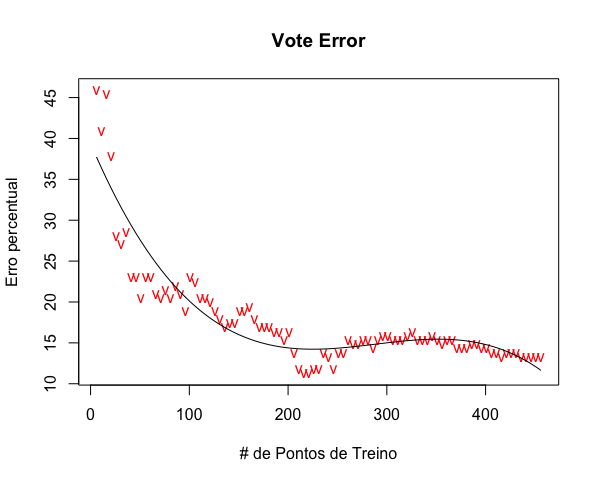
\includegraphics[scale=.55]{VoteError2zonesUCI}}






\bibliography{monografia}

%\appendix


\end{document}
